\documentclass[english]{article}

\usepackage[a4paper,margin=2cm]{geometry}
\usepackage{setspace}
\onehalfspacing

\usepackage{amsmath}
\usepackage{amsthm}
\usepackage{amssymb}

\usepackage{babel}

\usepackage{mathptmx}
\usepackage{amsmath}
\usepackage{graphicx}
\usepackage{color}

\newcommand{\Tr}{{\bf Tr}}
\newcommand{\R}{\mathbb{R}}
\newcommand{\E}{\mathbb{E}}
\newcommand{\N}{\mathcal{N}}
%\newcommand{\Pr}{ \text{Pr} }


\newtheorem{theorem}{Theorem}[section]
\newtheorem{conject}{Conjecture}[section]

\newtheorem{lemma}{Lemma}[section]
\newtheorem{corollary}{Corollary}[section]
\newtheorem{proposition}{Proposition}[section]


%% Choose one of the following (if not choosing the  
%% default, viz., Computer Modern, font family):
 %\usepackage{lmodern}
 %%
 %\usepackage{mathpazo}
% \usepackage[theoremfont]{newpxmath} \usepackage{newpxmath}
 %\usepackage{kpfonts}
 %%
 %\usepackage{mathptmx}
 %\usepackage{times,mtpro2}
 %\usepackage{stix}
 %\usepackage{txfonts}
 %\usepackage{newtxtext,newtxmath}
 %%
 
 %\usepackage{libertine} \usepackage[libertine]{newtxmath}
 
 %\usepackage{newpxtext} \usepackage[euler-digits]{eulervm}


\begin{document}


\title{Math 690 F2017: Topics in Data Analysis and Computation\\
Homework 1}

\author{Xiuyuan Cheng}

\date{}

\maketitle

\begin{enumerate}

\item
(Approximation and estimation error)
Consider the classification of numbers in $(-1,1)$, that is, 
$-1 <x  <1$ and $y=f(x)$ is the binary-valued function of class label, 
\[
f(x) = \begin{cases}
& 1,  \quad 0 \le  x < 1,\\
& 0,  \quad -1 <  x < 0.
\end{cases}
\]
Suppose that $x$ is uniformly distributed in $(-1,1)$. 

\begin{figure}[h]
\centering{
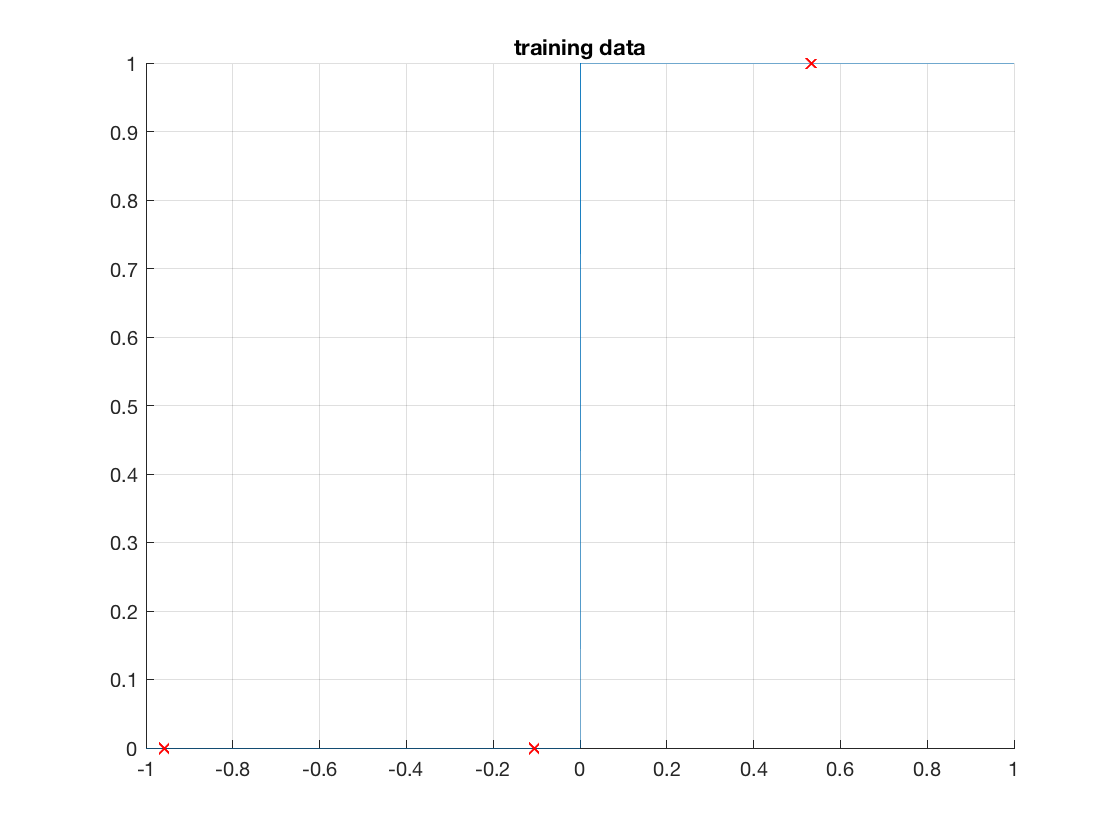
\includegraphics[width=0.6\linewidth]{hw1_1.png}
}
\caption{
The target classification function (blue line), and $n=3$ training samples (red cross).
}
\label{fig:1}
\end{figure}



Let $a > 0$ be a fixed constant,  $\sigma(x)=\frac{e^x}{ 1+ e^x}$ namely the ``sigmoid function".
Consider the class of models
\[
{\cal F}_a = \{ f_t(x) = \sigma\left(\frac{x-t}{a}\right), \, t\in (-1,1) \},
\]
which is a family of functions parametrized by one parameter $t$. $t$ stands for the location of the ``interface" where $f_t(x)$ transits from 0 to 1, and $a>0$ corresponds to the ``width" of the interface (plot it!). We firstly let $a=0.1$.

(1) What is the population (mean squared) loss for parameter $t$, which is 
\[
{\cal E} (t ) = \E |f_t(x) - f(x) |^2.
\]
Plot the function for $t \in (-1,1)$.

(2) Random draw $n=3$ i.i.d. training samples (an example shown in Figure \ref{fig:1}), consider the training error of model $f_t$ as a function of t,
\[
\hat{{\cal E}}(t ) = \frac{1}{3}\sum_{i=1}^3 |f_t(x_i)-f(x_i)|^2,
\]
plot the function for $t \in (-1,1)$. You can do it in the same figure as ${\cal E} (t )$  in (1) so as to compare.
Draw another set of $3$ training samples and see how the function $\hat{{\cal E}}(t )$ changes. 
What if $n=10$?

(3) Let $n=3$. Compute the minimizer of $\hat{{\cal E}}(t ) $. You can do it analytically or numerically, or use the following crude method: computing $\hat{{\cal E}}(t ) $ on a grid of values $t$, e.g. 100 evenly separated points in $(-1,1)$, and find the minimum on the grid. Then compute the error ${\cal E} (\hat{t} ) $ where $\hat{t}$ is the minimizer.
How is ${\cal E} (\hat{t} ) $  (expected testing error) compared with  $\hat{{\cal E}}(\hat{t}  ) $ (training error)?
Notice that $\hat{t}$ is a random variable (it is for the specific training set containing $n$ random samples), thus the two errors are random variables too.
Repeat the experiments for 100 times, and study the distribution of $\hat{{\cal E}}(\hat{t}  ) $  and ${\cal E} (\hat{t} ) $, e.g. the mean and variance.

(4) In (3), what is the difference of using the crude optimization compared to a more accurate optimization (e.g. the less crude optimization with 1000 grid point of $t$)?

(5) Repeat (3) and (4) for $n=10$.

(6) Repeat (1)-(5) for $a=0.01$ and compare to $a=0.1$, using a few different numbers of $n$, e.g. $n=3, 10, 20, \cdots$.
Compare the training and testing error for $a=0.1$ and $a=0.01$ with different $n$.
How large does $n$ need to be so that using $a=0.01$ leads to a better trained model, i.e. smaller (mean) ${\cal E}(\hat{t})$, than $a=0.1$?
(Hint: with $a=0.01$ the model function $f_t(x)$ has a sharper interface, which should better fit the target function if the correct $t$ can be found from data. You can plot the trained model $f_{\hat{t}}$ to see what it is like, over random draws of training set.) 

(7*) One can enlarge the model space by letting $a$ be a parameter as well, and then optimize over $\theta = (a,t)$. How will that affect the training the testing error? (Remark: by nature of this problem, the optimal $a$ which minimizes the training error will always be the smallest possible value in the optimization  - the sharpest interface is always the best to fit the discrete training data. However, from (6) we know that using sharp interface may lead to worse result due to limit number of training samples. To prevents $a$ being too small is an issue of regularization of the model.)


\end{enumerate}

\end{document}
